% =========================================================================== %
% Yes. This is a document.

\documentclass[
	english,
	aspectratio=169,
	table
]{beamer}

% =========================================================================== %
% Theme
\usepackage{scrlfile}
	\ReplacePackage{beamerthemeSHUR}{./sty/beamerthemeSHUR}
	\ReplacePackage{beamerinnerthemefancy}{./sty/beamerinnerthemefancy}
	\ReplacePackage{beamerouterthemedecolines}{./sty/beamerouterthemedecolines}
	\ReplacePackage{beamercolorthemechameleon}{./sty/beamercolorthemechameleon}

\usetheme[
	pageofpages=/,
	bullet=circle,
	titleline=true,
	alternativetitlepage=true,
	watermark="",
	watermarkheight=0px,
	watermarkheightmult=0
	]
{SHUR}

% =========================================================================== %
% the usual stuff

\usepackage[utf8]{inputenc}
\usepackage[T1]{fontenc}
\usepackage{babel}
\usepackage{lmodern}
\usepackage{microtype}
\usepackage{csquotes}
\usepackage{xspace}

\usepackage{tabularx}
\usepackage{booktabs}
\usepackage{multirow}

\usepackage{color, colortbl}
\usepackage{xcolor}
	\definecolor{tabhighlight}{RGB}{230,240,255}

\usepackage{tabto}

\usepackage{minted}
	\usemintedstyle{friendly}

\usepackage{tikz}
	\usetikzlibrary{positioning}
	\usetikzlibrary{matrix}
	\usetikzlibrary{shapes.geometric}
	\usetikzlibrary{backgrounds}
	\usetikzlibrary{calc}
	\usetikzlibrary{decorations.pathreplacing}
	\tikzstyle{every picture}+=[remember picture] 
\usepackage{adjustbox}

\usepackage{amsmath}
\usepackage{physics}

\usepackage[most]{tcolorbox}
	\tcbsetforeverylayer
		{colback=cyan!10!white,
		 colframe=cyan!75!black,
		 arc=0pt,
		 outer arc=0pt
		}
	\newtcolorbox{codebox}[1][Code]
		{colback=black!5!white,
		 colframe=blue!40!black,
		 title=#1,
		 leftupper=6mm
		}
	\newtcolorbox{cmdbox}[1][Command Line]
		{colback=black,
		 coltext=white,
		 fontupper=\ttfamily ,
		 colframe=blue!40!black,
		 title=#1,
		 outer arc=0pt
		}
	\newtcolorbox{warnbox}[1][Warning]
		{colback=black!5!white,
		 colframe=red!40!black,
		 title=#1
		}
	\newtcolorbox{hintbox}[1][Hint]
		{colback=black!5!white,
		 colframe=green!40!black,
		 title=#1
		}
	\newtcolorbox{defbox}[1][Code]
		{colback=cyan!10!white,
		 colframe=cyan!90!black,
		 title=#1
		}
%==============================================================================%
% GLOBAL MACROS

\newcommand*{\zB}{e.\,g. }
\newcommand*{\ie}{i.\,e. }

\newcommand{\Thus}{\ensuremath{\Rightarrow}\xspace}
\newcommand{\thus}{\ensuremath{\rightarrow}\xspace}

\newcommand*{\tabcrlf}{\\ \midrule}			% actually still allows for optional argument

\newcommand*{\inPy}[1]{\mintinline{python}{#1}}

\newcommand*{\todo}[1]{{\color{red}TODO: #1}}
\newcommand*{\sfrac}[2]{\ensuremath{{}^{#1}/_{#2}}}

% =========================================================================== %

\author{Stefan Hartinger}
\title{Python for Scientists}
\subtitle{Part 10: Handling Constants and Parameters}
\institute{Department of Just Some Dude Who Likes to Talk}
\date{Summer 2023}

% =========================================================================== %

\begin{document}
% =========================================================================== %

\begin{frame}[t,plain]
\titlepage
\end{frame}

% =========================================================================== %\\

\begin{frame}{Christmas Settings}
%
\begin{columns}[T]
\column{.5\linewidth}
\vspace{-12pt}
\begin{center}
	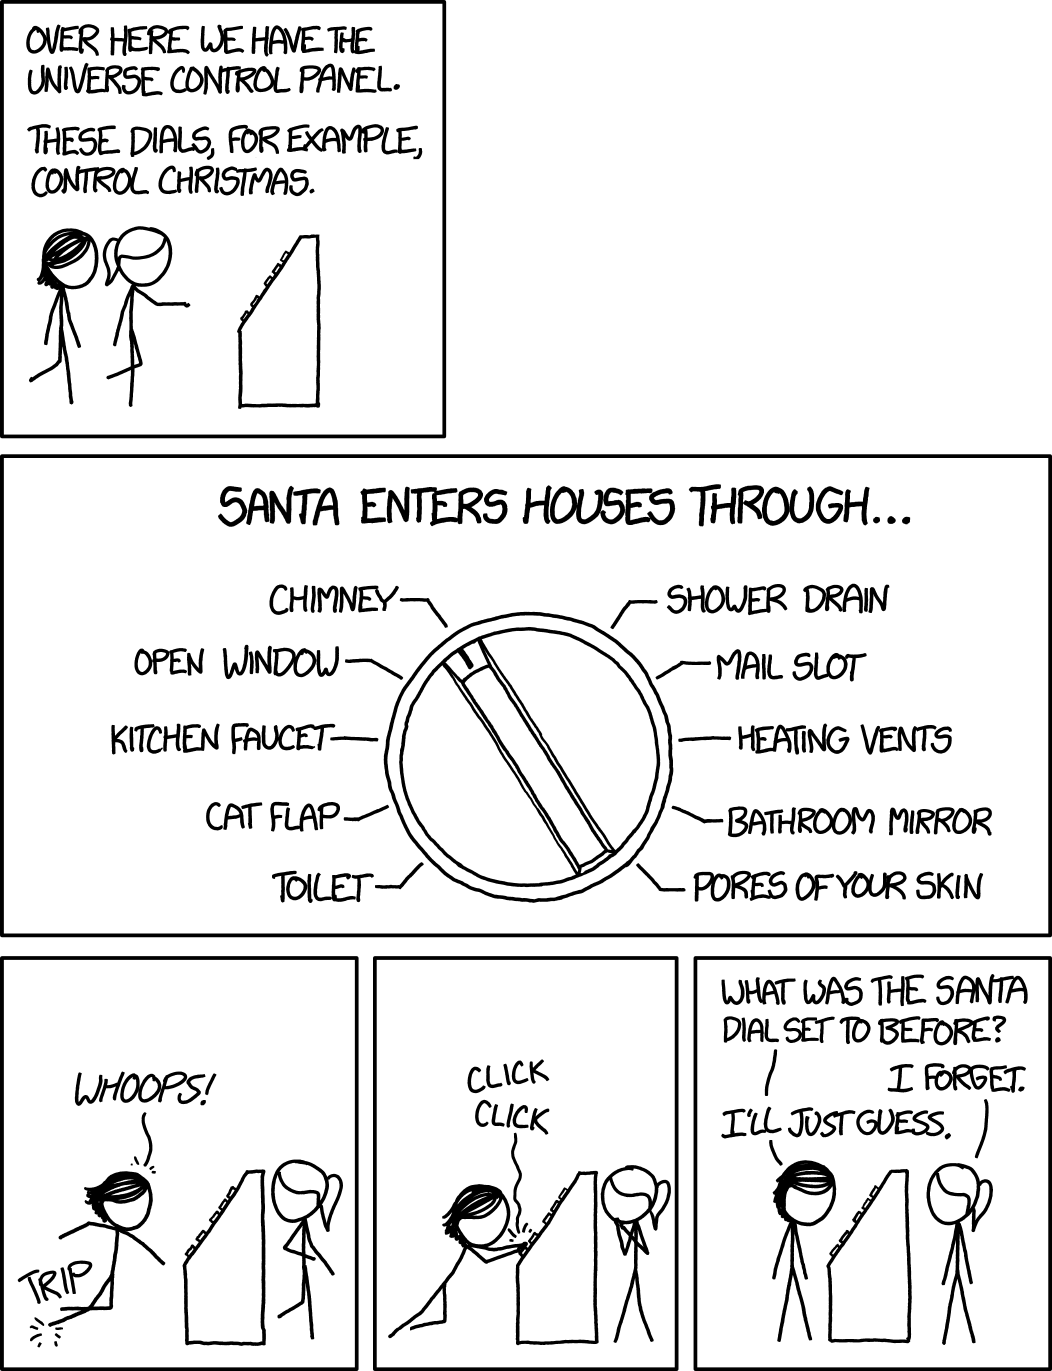
\includegraphics[width=.7\linewidth]{./gfx/10-xkcd-christmas-settings}
\end{center}
%
\column{.5\linewidth}
\vspace{+40pt}
\begin{center}
	\emph{SOUND DOGS MAKE: [BARKING] [HISSING] [LIGHTSABER NOISES] [FLUENT ENGLISH] [SWEARING]}
	
	\vspace{12pt}
	Source: \url{https://xkcd.com/1620/}
\end{center}
\end{columns}
%
\end{frame}

% =========================================================================== %

\begin{frame}{A Problem From My Master Thesis}
%
\begin{center}
\tiny
(and a billion other projects, too)
\end{center}
%
\begin{itemize}
\item Handle (universal) constants, session constants and global variables
	\begin{itemize}
	\item To my knowledge, the terms \emph{universal constants} and \emph{session constants} are no fixed terms.
	\item For this presentation, it makes sense to introduce the names as they behave a bit differently
	\end{itemize}
\item (Universal) constants: true constants like $\pi$, $\hbar, ...$
\item Session constants: could have any value, but constant within one run of a simulation. E.\;g. $N_{\text{photons}}$, $t_{\text{timeout}}$, ...
\item Global variables: well, they're variable and they are available from anywhere in the code...
	\begin{itemize}
	\item The dogma is to \emph{generally avoid} globals, but at any cost
	\item In fact, session constants, for example, are often implemented as global variables: \\
		Set their value in an initialization phase (\emph{at runtime!}) \Thus \emph{variables}\\
		Treat them as constants after that \Thus \emph{globals}
	\end{itemize}
\end{itemize}
%
\end{frame}

% =========================================================================== %

\begin{frame}{My Preferred Model}
%
\begin{center}
\tiny
(and that of a lot of other coders, too)
\end{center}
%
\begin{itemize}
\item Have a dedicated module \texttt{globals.py} that stores both, universal and session constants
\item Universal constants are simply set as literal values in \texttt{globals.py}
\item Session constants come from two \emph{external} sources
	\begin{itemize}
	\item A settings file (\texttt{settings.ini})
	\item The command line parameters \\
		\texttt{python3 mySimulation.py highResolutionScan.ini -{}-debug}
	\end{itemize}
\item This split between settings file and command line parameters allows to ...
	\begin{itemize}
	\item ... store results with inputs but separate from the code
	\item ... distinguish between rarely changed and more volatile parameters
	\end{itemize}
\end{itemize}
%
\begin{hintbox}[Matter of taste]
\footnotesize
Of course, you can also use a settings file without command line parameters and vice versa.
\end{hintbox}
%
\end{frame}

% =========================================================================== %

\begin{frame}{Scope For Today}
%
\begin{itemize}
\item Module Mechanics
	\begin{itemize}
	\item Initialization
	\item Mutability
	\end{itemize}
\item The module \texttt{argparse}
	\begin{itemize}
	\item How to access command line parameters in the first place
	\item Conventions and Variations (why you want a pre-made parser)
	\item How to use \texttt{argparse}
	\end{itemize}
\item The module \texttt{configparser}
	\begin{itemize}
	\item The \texttt{.ini} format
	\item Using \texttt{configparser}
	\item Type Conversion and Fallback Values
	\item Interpolation
	\end{itemize}
\item Coding Guideline: Fail Fast
\end{itemize}
%
\end{frame}

% =========================================================================== %

\begin{frame}[fragile]
%
\vspace{-12pt}
\begin{columns}[T]
\column{.46\linewidth}
\begin{codebox}[Example: main.py]
\begin{minted}[linenos, fontsize=\scriptsize]{python3}
import Constants
import Utility

print("Main (before):",
      Constants.Value)

Constants.Value = 1337

print("Main (after):",
       Constants.Value)

Utility.show_constants()
\end{minted}
\end{codebox}
%
\column{.47\linewidth}
\begin{codebox}[Example: Constants.py]
\begin{minted}[linenos, fontsize=\scriptsize]{python3}
print("Initializing Constants ...",
      end="")
Value = 1989
print(" done")
\end{minted}
\end{codebox}
%
\vspace{-10pt}
\begin{codebox}[Example: Utility.py]
\begin{minted}[linenos, fontsize=\scriptsize]{python3}
import Constants

def show_constants():
    print("Utility:", Constants.Value)
\end{minted}
\end{codebox}
\end{columns}
%
\vspace{-4pt}
\begin{cmdbox}[Output]
\begin{minted}[fontsize=\scriptsize]{text}
Initializing Constants ... done
Main (before): 1989
Main (after): 1337
Utility: 1989
\end{minted}
\end{cmdbox}
%
\end{frame}

% =========================================================================== %

\begin{frame}{Interpretation}
%
\begin{itemize}
\item Truly Constant Values
	\begin{itemize}
	\item do not exist in Python :(
	\item Convention: ALL CAPS symbols are meant to be read only
	\end{itemize}
\item Order Of Execution
	\begin{itemize}
	\item \texttt{Constants.py} is \inPy{import}ed twice
	\item But we see \texttt{Initializing Constants ... done} only once
	\item[\Thus] Python keeps track which modules are already in memory and initialized
	\item[\Thus] \inPy{import} in \texttt{Utility.py} still necessary to make symbols visible
	\end{itemize}
\item Changing Values
	\begin{itemize}
	\item Possible within \texttt{main.py} but effect does not propagate into \texttt{Utility.py}?
	\item Because Value is of class \inPy{str}ing and thus is \emph{immutable}!
	\item[\Thus] Rebinding in \texttt{main.py}, but not really reassiging the value
	\end{itemize}
\end{itemize}
%
\end{frame}

% =========================================================================== %

\begin{frame}{Getting Around this Limitation}
%
\begin{itemize}
\item Put all global objects into a mutable container
	\begin{itemize}
	\item Like a \inPy{dict}
		\begin{itemize}
		\item \inPy{Constants = {"Value" : 1989, "Foo" : "Bar", ...}}
		\item Verbose access \texttt{Constants.Constants["Value"]}
		\item[\Thus] \inPy{from Constants import Constants} 
		\item Quick and dirty, but there's a better way
		\end{itemize}
	\end{itemize}
\item Put all global objects into a \inPy{class}
	\begin{itemize}
	\item Easiest: simply use the class attributes
	\item Sometimes better: instantiate the class
	\end{itemize}
\end{itemize}
%
\end{frame}

% =========================================================================== %

\begin{frame}[fragile]
%
\vspace{-12pt}
\begin{columns}[T]
\column{.46\linewidth}
\begin{codebox}[Example: main.py]
\begin{minted}[linenos, fontsize=\scriptsize]{python3}
from Constants import Constants
import Utility

print("Main (before):",
      Constants.Value)

Constants.Value = 1337

print("Main (after):",
       Constants.Value)

Utility.show_constants()
\end{minted}
\end{codebox}
%
\column{.47\linewidth}
\begin{codebox}[Example: Constants.py]
\begin{minted}[linenos, fontsize=\scriptsize]{python3}
print("Initializing Constants")
class Constants:
    Value = 1989
    ...
\end{minted}
\end{codebox}
%
\vspace{-10pt}
\begin{codebox}[Example: Utility.py]
\begin{minted}[linenos, fontsize=\scriptsize]{python3}
from Constants import Constants

def show_constants():
    print("Utility:", Constants.Value)
\end{minted}
\end{codebox}
\end{columns}
%
\vspace{-4pt}
\begin{cmdbox}[Output]
\begin{minted}[fontsize=\scriptsize]{text}
Initializing Constants
Main (before): 1989
Main (after): 1337
Utility: 1337
\end{minted}
\end{cmdbox}
%
\end{frame}

% =========================================================================== %

\begin{frame}[fragile]{Problems With That Approach}
%
\vspace{-9pt}
\begin{warnbox}[Cross-Referencing Constants, leftupper=7mm]
\begin{minted}[linenos, fontsize=\scriptsize]{python3}
class Constants:
    VERSION = "1.0"
    SIGNATURE = f"Library v{Constants.VERSION}"
\end{minted}
\end{warnbox}
%
\begin{itemize}
\item Results in a \texttt{NameError}
\item Class \texttt{Constants} is not completed when it's referred to the first time
\end{itemize}
%
\begin{codebox}[Solution: Postponing The Access]
\begin{minted}[linenos, fontsize=\scriptsize]{python3}
class Constants:
    VERSION = "1.0"
    SIGNATURE = None

Constants.SIGNATURE = f"Library v{Constants.VERSION}"
\end{minted}
\end{codebox}
%
\end{frame}

% =========================================================================== %

\begin{frame}[fragile]{Atlernative: Instantiation}
%
\vspace{-9pt}
\begin{codebox}[Constants.py]
\begin{minted}[linenos, fontsize=\scriptsize]{python3}
class ConstantsClass:
    def __init__(self)
        self.VERSION = "1.0"
        self.SIGNATURE = f"Library v{Constants.VERSION}"

Constants = ConstantsClass()
\end{minted}
\end{codebox}
%
\begin{codebox}[main.py]
\begin{minted}[linenos, fontsize=\scriptsize]{python3}
from Constants import Constants

if __name__ == "__main__":
    print(Constants.SIGNATURE)
\end{minted}
\end{codebox}
%
Or: Use \emph{Singleton} Pattern!
%
\end{frame}

% =========================================================================== %

\begin{frame}{In Comparison}
%
\begin{itemize}
\item Module level constants
	\begin{itemize}
	\item Least overhead
	\item Cause problems when changed at runtime
	\end{itemize}
\item Class attributes
	\begin{itemize}
	\item Simple way of making all objects mutable
	\item Cause problems when constants reference each other
	\end{itemize}
\item Instantiation
	\begin{itemize}
	\item Highest level of flexibility
	\item Some mental overload -- dealing with class or with member?
	\item Allows neat tricks (more easily)
	\end{itemize}
\end{itemize}
%
\begin{hintbox}[A Matter Of Scope And Taste]
\footnotesize
All of the above are valid patterns. What you actually implement depends on your needs and taste.
\end{hintbox}
%
\end{frame}

% =========================================================================== %

\begin{frame}{Command Line Arguments}
%
\begin{itemize}
\item Remember: The command line interpreter (CLI) can pass on information to the executed program
\item When running a Python script: anything \emph{behind} the \texttt{.py} file will be sent to the script as parameter
\item Example:
	\begin{itemize}
	\item \texttt{python3 -b myScript.py arg1 arg2 "arg3 with whitespaces"}
	\item \texttt{-b} is a parameter for the Python interpreter itself (extra warnings for suspicious conversions \inPy{bytes} \thus \inPy{str})
	\item \texttt{arg1}, \texttt{arg2}, ... are parameters for the \texttt{myScript.py}
	\item Parameters are split at whitespaces, unless enclosed in \texttt{"}double quotes\texttt{"}
	\end{itemize}
\item To access these parameters in code, ...
	\begin{itemize}
	\item \inPy{import sys}
	\item Read the \inPy{list sys.argv}
	\item \inPy{sys.argv[0]} holds the script name (\zB \texttt{some/path/myScript.py})
	\item The other elements are \inPy{"arg1"} \inPy{"arg2"} and \inPy{"arg3 with whitespaces"}, respectively
	\end{itemize}
\end{itemize}
%
\end{frame}

% =========================================================================== %

\begin{frame}{Conventions}
%
\begin{itemize}
\item There can be positional/mandatory parameters as well as optional parameters
\item The order of optional parameters is not important but specified by a keyword
\item Optional parameters have a prefix hyphen (\zB \texttt{program -d})
	\begin{itemize}
	\item A single hyphen indicates the short form (one character) of the parameter
	\item The long form has a double hyphen and is a multi-character word, \\
		like in \texttt{program -{}-debug}
	\item Abbreviations should also work (\texttt{program -d} is equivalent to \texttt{program -{}-debug})
	\end{itemize}
\item Optional parameters may be booleans (like \texttt{-{}-debug}) or have one or several values
	\begin{itemize}
	\item E.\;g. \texttt{program -{}-n\_processes 4} 
	\item E.\;g. \texttt{program -{}-headers foo bar baz -{}-debug}
	\end{itemize}
\item Invocation with \texttt{-h} or with \texttt{-{}-help} shows help
\end{itemize}
%
\begin{warnbox}[Do Not Re-Invent The Wheel]
\footnotesize
It is of course possible to implement all of that (and more) in Python yourself -- argparse is written in Python -- but would waste a lot of time.
\end{warnbox}
%
\end{frame}

% =========================================================================== %

\begin{frame}[fragile]{The basics of \texttt{argparse}}
%
\begin{itemize}
\item Instantiate a parser
	\begin{itemize}
	\item \inPy{parser = argparse.ArgumentParser(description="what the program does")}
	\item The string \texttt{description} is used for the help text.
	\item There are more options to the constructor -- see online documentation
	\end{itemize}
\item Add parameters with options (see next slides)
	\begin{itemize}
	\item \inPy{parser.add_argument("settingsfile")} -- expects one string \\
		(\zB \texttt{program settings.ini})
	\item \inPy{parser.add_argument("--logfile")}  -- expects one optional string after keyword \\
		(\zB \texttt{program -{}-logfile name.log} or simply omit: \texttt{program})
	\end{itemize}
\item Run the parser
	\begin{itemize}
	\item \texttt{cli\_params = parser.parse\_args()}
	\item Automatically aborts if mandatory parameters missing or other rules violated
	\item Automatically prints error message or help text
	\end{itemize}
\item Use the results like attributes: \inPy{if cli_params.debug: ...}
\end{itemize}
%
\end{frame}

% =========================================================================== %

\begin{frame}[fragile]{More About \texttt{add\_argument}}
%
\begin{itemize}
\item Takes one or more strings that specify the name of an argument
\item The first full length name will be the one usable in code
	\begin{itemize}
	\item Full length: qualified by a double hyphen (or no hyphen at all)
	\item E.\;g. \inPy{parser.add_argument("--foo", "--bar")}
	\item[\Thus] You can start with \texttt{program.py --foo value} or \texttt{program.py --bar value}
	\item[\Thus] But, in code, only \texttt{cli\_params.foo} will exist (and stores \inPy{"value"})
	\item ... unless you specify your own name with the keyword argument \texttt{dest}
	\item[\Thus] \inPy{parser.add_argument("--foo", "--bar", dest="nameInCode")}
	\end{itemize}
\item Omitted optional arguments will be \inPy{None}
	\begin{itemize}
	\item ... unless you specify a default value
	\item[\Thus] \inPy{parser.add_argument("--settings", default="settings.ini")}
	\end{itemize}
\item Add a description for each argument with the \texttt{help} keyword
	\begin{itemize}
	\item [\Thus] \inPy{parser.add_argument("--settings", help="which settings to use")}
	\end{itemize}
\end{itemize}
%
\end{frame}

% =========================================================================== %

\begin{frame}[fragile]{Even More About \texttt{add\_argument}}
%
\begin{itemize}
\item You can specify several behaviors with the \texttt{action} and \texttt{const}, of which the most important ones are
	\begin{itemize}
	\item \inPy{action="store_const"} -- if flag is present, store \texttt{const} in result variable
	\item \inPy{action="store_true"} -- short form for \inPy{action="store_const", default=False, const=True}
	\item \inPy{action="store_false"} -- likewise, values flipped
	\item \inPy{action="count"} -- counts how often the flag appears in the call
	\item If \inPy{parser.add_argument("-v", action="count")}, \texttt{program.py -vvv}  gives \texttt{3}
	\end{itemize}
\item Number of arguments for a given keyword can be controlled with \texttt{nargs}
	\begin{itemize}
	\item \inPy{parser.add_argument("--foo", nargs=2)}
	\item You can also put special strings here:
		\begin{itemize}
		\item \inPy{"*"} -- any number of arguments (result is a \inPy{list} of strings)
		\item \inPy{"+"} -- at least one argument (result is a \inPy{list} of strings)
		\item \inPy{"?"} -- one or zero arguments for non-hyphenated arguments; use \texttt{const} for hyphenated arguments without value
		\end{itemize}
	\end{itemize}
\end{itemize}
%
\end{frame}

% =========================================================================== %

\begin{frame}[fragile]{Still Not Everything About \texttt{add\_argument}}
%
\begin{itemize}
\item Limit the range of valid parameters with the \texttt{choices} keyword
	\begin{itemize}
	\item \inPy{parser.add_argument("--doc", choices=["death", "cake"])}
	\item Eddie Izzard: \emph{Dress to Kill} (\url{https://www.youtube.com/watch?v=PVH0gZO5lq0})
	\end{itemize}
\item Convert to a specific type with the \texttt{type} keyword
	\begin{itemize}
	\item String from CLI will be passed to the type's constructor
	\item \inPy{parser.add_argument("--n_processes", type=int)}
	\end{itemize}
\item Add a description for what each parameter does with the \texttt{help} keyword
\item Of course, all of them can be used in combination
\item More: See \url{https://docs.python.org/3/library/argparse.html}
\end{itemize}
%
\end{frame}

% =========================================================================== %

\begin{frame}[fragile]
%
\begin{codebox}[Globals.py]
\begin{minted}[linenos, fontsize=\scriptsize]{python3}
class GlobalsClass:
    def __init__(self)
        self.CLI_ARGUMENTS = None
        ...
        self.parse_command_line()

    def parse_command_line(self):
        parser = argparse.ArgumentParser(description="runs a simulation")

        parser.add_argument("inputFiles", nargs="+")
        parser.add_argument("--logfile", help="redirects output to a file")
        parser.add_argument("--settings", default="settings.ini")
        parser.add_argument("--debug", action='store_true')

        self.CLI_ARGUMENTS = parser.parse_args()

Globals = GlobalsClass()

# later access Globals.CLI_ARGUMENTS.debug, etc.
\end{minted}
\end{codebox}
%
\end{frame}

% =========================================================================== %

\begin{frame}[fragile]
%
\begin{cmdbox}[Execution Examples]
\begin{minted}[fontsize=\scriptsize]{text}
$ python3 simulation.py --help
usage: simulation.py [-h] [--logfile LOGFILE] [--settings SETTINGS] [--debug]
               inputFiles [inputFiles ...]

runs a simulation

positional arguments:
  inputFiles

options:
  -h, --help           show this help message and exit
  --logfile LOGFILE    redirects output to a file
  --settings SETTINGS
  --debug

$ python3 simulation.py 
usage: simulation.py [-h] [--logfile LOGFILE] [--settings SETTINGS] [--debug]
               inputFiles [inputFiles ...]
main.py: error: the following arguments are required: inputFiles

\end{minted}
\end{cmdbox}
%
\end{frame}

% =========================================================================== %

\begin{frame}{The \texttt{.ini} Format}
%
\begin{itemize}
\item Keyword-Value-Pairs, separated by equals sign or colon
	\begin{itemize}
	\item \texttt{N\_photons = 4}
	\item \texttt{enable\_advanced\_filter : On}
	\end{itemize}
\item Allows Comments with either semicolon or pound symbol
	\begin{itemize}
	\item \texttt{\# advanced filter also detects tachyon interference}
	\item \texttt{; advanced filter also detects tachyon interference}
	\item May be indented, but not part of a parameter definition
	\item[\Thus] This will not work: \\
		\texttt{N\_photons = 4; only even numbers valid} 
	\end{itemize}
\item Multiple sections, derived from a possibly implicit \texttt{DEFAULT} section
	\begin{itemize}
	\item Section: Namespace, grouping of parameters
	\item Let there be \texttt{Section\_A} and \texttt{Section\_B} each with parameters \texttt{X}, \texttt{Y}, \texttt{Z}
	\item Then you get to have a \texttt{Section\_A.X} which can be different from \texttt{Section\_B.X}, etc.
	\item A value \texttt{DEFAULT.D} also exists as \texttt{Section\_A.D}, unless explicitly overwritten
	\item No nested sections allowed
	\end{itemize}
\end{itemize}
%
\end{frame}

% =========================================================================== %

\begin{frame}[fragile]
%
\begin{codebox}[Example ini File]
\begin{minted}[linenos, fontsize=\scriptsize]{ini}
[DEFAULT]
username = has13223
machine = rex1
localdir = ./
serverdir = ~/
server = uni-regensburg.de
shell = bash

[workgroup]
machine = pc123456789
serverdir = /local/hartinger/
\end{minted}
\end{codebox}
%
\begin{hintbox}[Context]
\footnotesize
I used this in a tool to exchange files between my personal computer and various UR machines via ssh/scp. Default communication should happen on the machine rex1, but a command like \\
\texttt{remote push myFile --preset workgroup} \\
should use a different set of parameters.
\end{hintbox}
%
\end{frame}

% =========================================================================== %

\begin{frame}{Using \texttt{configparser}}
%
\begin{itemize}
\item Instantiate a parser:\\
	\texttt{config = configparser.ConfigParser()}
\item Run it on a file:\\
	\texttt{config.read(settings\_file)}
\item Access the items ...
	\begin{itemize}
	\item like a (nested) dict: \\
		\inPy{config["DEFAULT"]["username"]}
	\item or with method \texttt{get} to provide fallback values if the file does not contain the parameter: \\
		\inPy{config.get("workgroup.password", "foo bar")}
	\end{itemize}
\end{itemize}
%
\begin{warnbox}[Never store passwords in clear text files]
\footnotesize
Neither in \texttt{.ini} files nor in your code. Just don't do it.
\end{warnbox}
%
\end{frame}

% =========================================================================== %

\begin{frame}{Some Extras In \texttt{configparser}}
%
\begin{itemize}
\item Data Types
	\begin{itemize}
	\item By Default: Everything is a \inPy{str}ing
	\item \inPy{parser["section"].getboolean("key")} -- returns a \inPy{boolean} and recognizes \texttt{true/false}, \texttt{on/off}, \texttt{yes/no} and \texttt{1/0}
	\item Likewise: \texttt{getint} and \texttt{getfloat}
	\end{itemize}
\item Checking if a parameter is in the settings file
	\begin{itemize}
	\item \inPy{"parameter" in parser["section"]} returns \inPy{True} or \inPy{False}
	\end{itemize}
\item Iterating over all parameters in a section
	\begin{itemize}
	\item \inPy{for parameter in parser: ...}
	\item Includes parameters in \texttt{DEFAULT} section
	\end{itemize}
\item Writing a configuration back to disk
	\begin{itemize}
	\item \texttt{parser.write(fileobject)}
	\item \texttt{fileobject} is a file handle (the return value from an \inPy{open} call)
	\end{itemize}
\end{itemize}
%
\end{frame}

% =========================================================================== %

\begin{frame}{More About \texttt{configparser}}
%
\begin{itemize}
\item Case sensitivity
	\begin{itemize}
	\item Sections are case sensitive
	\item Parameter names are not (by default)
	\item See \texttt{optionxform} on \url{https://docs.python.org/3/library/configparser.html} for details
	\end{itemize}
\item Empty vs. non-existent parameters
	\begin{itemize}
	\item Empty value: \texttt{parameter} without \texttt{= value}; evaluates to \inPy{None}
	\item Null-String: \texttt{parameter=}; evaluates to \inPy{""}
	\item Not in \texttt{.ini} file at all: raises \inPy{KeyError} (unless accessed with \texttt{get} and fallback value)
	\end{itemize}
\item Indents
	\begin{itemize}
	\item Leading Whitespaces before sections, parameter keys or comments are ignored
	\end{itemize}
\item Multiline values
	\begin{itemize}
	\item Possible
	\item The second to last lines need to be indented wrt. the first line
	\end{itemize}
\end{itemize}
%
\end{frame}

% =========================================================================== %

\begin{frame}[fragile]{Interpolation}
%
\begin{itemize}
\item \texttt{.ini} file parameters can reference each other, recursively
\item Example:
	\begin{minted}[fontsize=\scriptsize]{ini}
	[Paths]
	home_dir: /Users
	my_dir: %(home_dir)s/lumberjack
	my_pictures: %(my_dir)s/Pictures
	\end{minted}
\item \texttt{\%(} marks beginning of referenced object, \texttt{)s} marks the end
\item The string in between is a key name of the current section and will be replaced by its respective key value
\item In the above example: \texttt{my\_pictures = /Users/lumberjack/Pictures}
\item To encode value \texttt{\%}: Escape with double percent sign (\texttt{key = \%\%}) ...
\item ... or deactivate interpolation alltogether: \\
	\inPy{parser = configparser.ConfigParser(interpolation=None)}
\end{itemize}
%
\end{frame}

% =========================================================================== %

\begin{frame}{Coding Guideline: Fail Fast}
%
\begin{itemize}
\item Temptation: Provide Default values for everything
\item Seemingly improves comfort for user, but also adds pitfals
\item Are default values intuitive for user?
\item Are they compatible with all inputs?
\item[\Thus] Provide them where they are safe to use, but ...
\item[\Thus] ... do not be afraid to tell your user they've forgotten some vital information
\end{itemize}
%
\begin{hintbox}[Check Availability of Needed Information in Initialization Phase]
\footnotesize
Do not guard access to the parameters mid-algorithm! Rather, check if everything is ready before you start your \enquote{proper} code. Not only with that pattern you can't forget a guard clause; also your user directly receives feedback and doesn't have to wait through part of a simulation before they get the error message.
\end{hintbox}
%
\end{frame}

\end{document}

% MAREI!!
% whom do I give credit? Where?